\input{../../headers/tdheaders.tex}

\newpage

\section{Moteur à explosion}

\subsection{Mise en situation}

\begin{figure}[htbp]
\begin{minipage}[c]{.4\linewidth}
\begin{center}
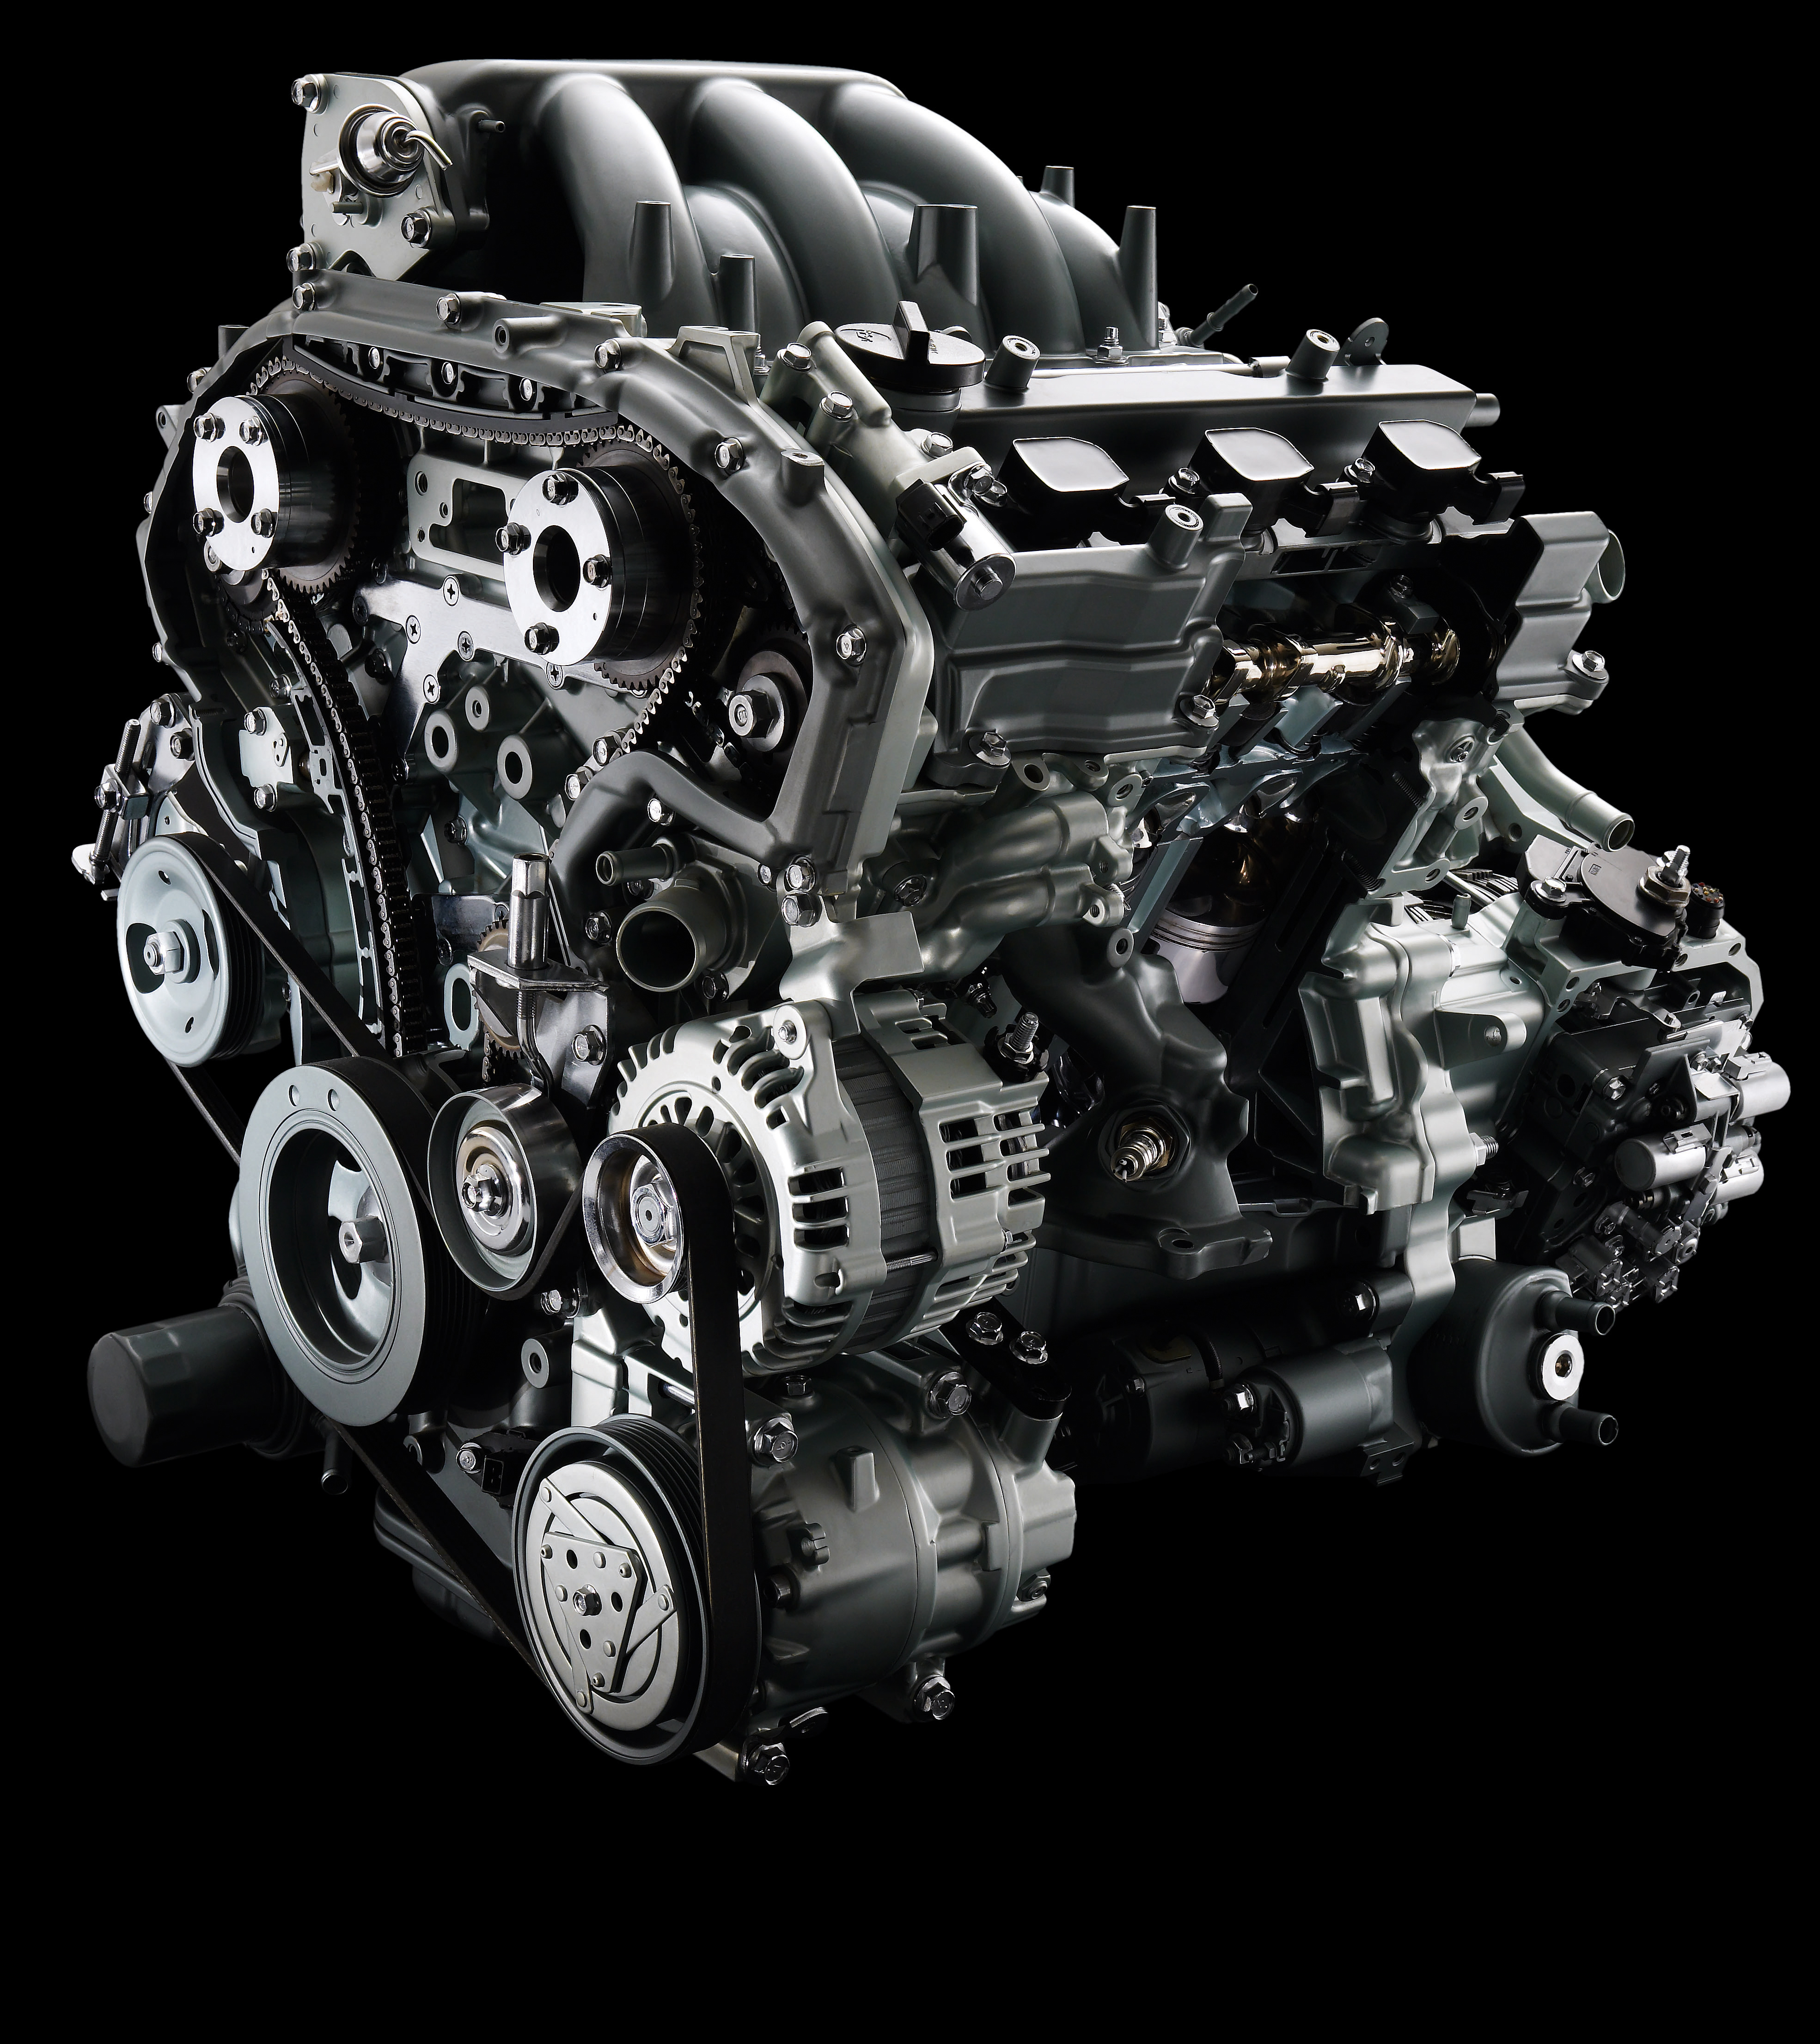
\includegraphics[width=\linewidth]{img/moteur_laguna.jpg}
\caption{Moteur de Renault Laguna}
\label{fig:image8}
\end{center}
\end{minipage}
\hfill
\begin{minipage}[c]{.55\linewidth}
Le moteur à explosion est un type de moteur à combustion interne, il est principalement utilisé pour la propulsion des véhicules de transport (avion à hélice, automobile, moto, camion, bateau), ainsi que pour une multitude d'outils mobiles (tronçonneuse, tondeuse à gazon) ainsi que pour des installations fixes (groupe électrogène, pompe).

Le terme moteur à explosion, consacré par l'usage est impropre car il ne rend pas compte de tous les phénomènes se produisant dans ces moteurs, pour lesquels la dénomination à combustion interne est nettement plus adéquate.
\end{minipage}
\end{figure}

\subsection{Présentation du système}

Le cycle de fonctionnement se décompose de manière analytique en quatre temps ou phases. Le mouvement du piston est initié par la combustion (augmentation rapide de la température et donc de la pression des gaz) d'un mélange de carburant et d'air (comburant) qui a lieu durant le temps moteur. C'est le seul temps produisant de l'énergie ; les trois autres temps en consomment mais le rendent possible.

Le piston se déplace pendant le démarrage grâce à une source d'énergie externe (souvent un démarreur ou lanceur : un moteur électrique est couplé temporairement au vilebrequin) jusqu'à ce qu'au moins un temps moteur produise une force capable d'assurer les trois autres temps avant le prochain temps moteur. Le moteur fonctionne dès lors seul et produit un couple sur son arbre de sortie.

Voici une description des cycles successifs d'un moteur à quatre temps :

\begin{itemize}
 \item admission d'un mélange air et de carburant vaporisé, présent dans le conduit d'admission, mélange préparé par divers composants (carburateur ou système d'injection indirecte) : ouverture de la soupape d'admission et descente du piston, ce dernier aspire ainsi ce mélange dans le cylindre à une pression de -0,1 à -0,3 bar ;
 \item compression du mélange : fermeture de la soupape d'admission, puis remontée du piston qui comprime le mélange jusqu'à 30 bars et 400 à 500 °C dans la chambre de combustion ;
 \item combustion et détente aux environs du point mort haut : moment auquel le piston atteint son point culminant et auquel la compression est au maximum ; la bougie d'allumage, connectée à un générateur d'électricité haute tension, produit une étincelle ; la combustion rapide qui s'ensuit constitue le temps moteur ; les gaz chauds à une pression de 40 à 60 bars repoussent le piston, initiant le mouvement ;
 \item échappement : ouverture de la soupape d'échappement et remontée du piston qui chasse les gaz brûlés détendus dans le collecteur d'échappement.
\end{itemize}

Et un nouveau cycle commence en 1.

\begin{figure}[htbp]
\begin{center}
 \includegraphics[width=\linewidth]{img/cycles.jpg}
\caption{Cycle de Beau de Rochas}
\label{fig:image9}
\end{center}
\end{figure}

Le \textbf{vilebrequin} (1) est en liaison avec le \textbf{carter} (0) au point $A$. La \textbf{bielle} (2) est en liaison avec le \textbf{vilebrequin} au point $B$. Le \textbf{piston} (3) est en liaison avec la bielle au point $C$.

\paragraph{Question 1:} Réaliser le graphe de liaison de ce mécanisme. Donner, pour chaque liaison, le type de liaison, le point d'application ainsi que le ou les axes nécessaires à sa description.

\paragraph{Question 2:} Représentez le mécanisme du moteur à l'aide d'un schéma cinématique.

\paragraph{Question 3:} Écrire le torseur de chacune de ces liaisons à son point d'application.

\paragraph{Question 4:} Paramétrer le schéma cinématique en y incluant les centres des liaisons ainsi que les repères des pièces.

~\

La loi de composition des vitesses nous donne les équations suivantes:
\begin{itemize}
 \item $\overrightarrow{V_{C\in 3/0}}=\overrightarrow{V_{C\in 3/2}}+\overrightarrow{V_{C\in 2/1}}+\overrightarrow{V_{C\in 1/0}}$,
 \item $\overrightarrow{\Omega_{3/0}}=\overrightarrow{\Omega_{3/2}}+\overrightarrow{\Omega_{2/1}}+\overrightarrow{\Omega_{1/0}}$.
\end{itemize}

\paragraph{Question 5:} En utilisant le théorème de Varignon, déterminer $\overrightarrow{V_{C\in 3/2}}$, $\overrightarrow{V_{C\in 2/1}}$ et $\overrightarrow{V_{C\in 1/0}}$.

\paragraph{Question 6:} En utilisant la loi de composition des vitesses, déterminer $\overrightarrow{V_{C\in 3/0}}$.

\paragraph{Question 7:} En utilisant l'architecture du système, proposer une simplification de l'écriture de $\overrightarrow{V_{C\in 3/0}}$.

\paragraph{Question 8:} En déduire la norme de $\overrightarrow{V_{C\in 3/0}}$ en fonction des normes des vitesses de rotation $\overrightarrow{\Omega_{3/0}}$, $\overrightarrow{\Omega_{3/2}}$, $\overrightarrow{\Omega_{2/1}}$, $\overrightarrow{\Omega_{1/0}}$.


\section{La chaise de dentiste: Bac STI (GE) 2006}

\subsection{Mise en situation}

\begin{figure}[htbp]
\begin{minipage}[c]{.4\linewidth}
\begin{center}
\includegraphics[width=\linewidth]{img/cabinet.jpg}
\caption{Fauteuil dans un cabinet}
\label{fig:image1}
\end{center}
\end{minipage}
\hfill
\begin{minipage}[c]{.55\linewidth}
La chirurgie dentaire et ses spécificités opératoires nécessitent l'installation du patient dans une position couchée particulière (voir illustration ci-dessous). La société AIREL a donc développé un fauteuil d'opération ergonomique, véritable automate comportant toutes les commandes et les fonctions dont le praticien doit disposer, quelle que soit sa spécialité et ses contraintes opératoires.
\end{minipage}
\end{figure}

\subsection{Présentation du système}

\begin{figure}[htbp]
\begin{minipage}[c]{.5\linewidth}
Le système de levée du fauteuil, qui va être l'objet de notre étude, est composé d'un vérin ainsi que d'un système pantographe.

Il permet de piloter la montée et la descente du fauteuil afin de placer le patient à une hauteur adéquate afin que le médecin pratique son intervention dans les meilleures conditions possibles.
\end{minipage}
\hfill
\begin{minipage}[c]{.45\linewidth}
\begin{center}
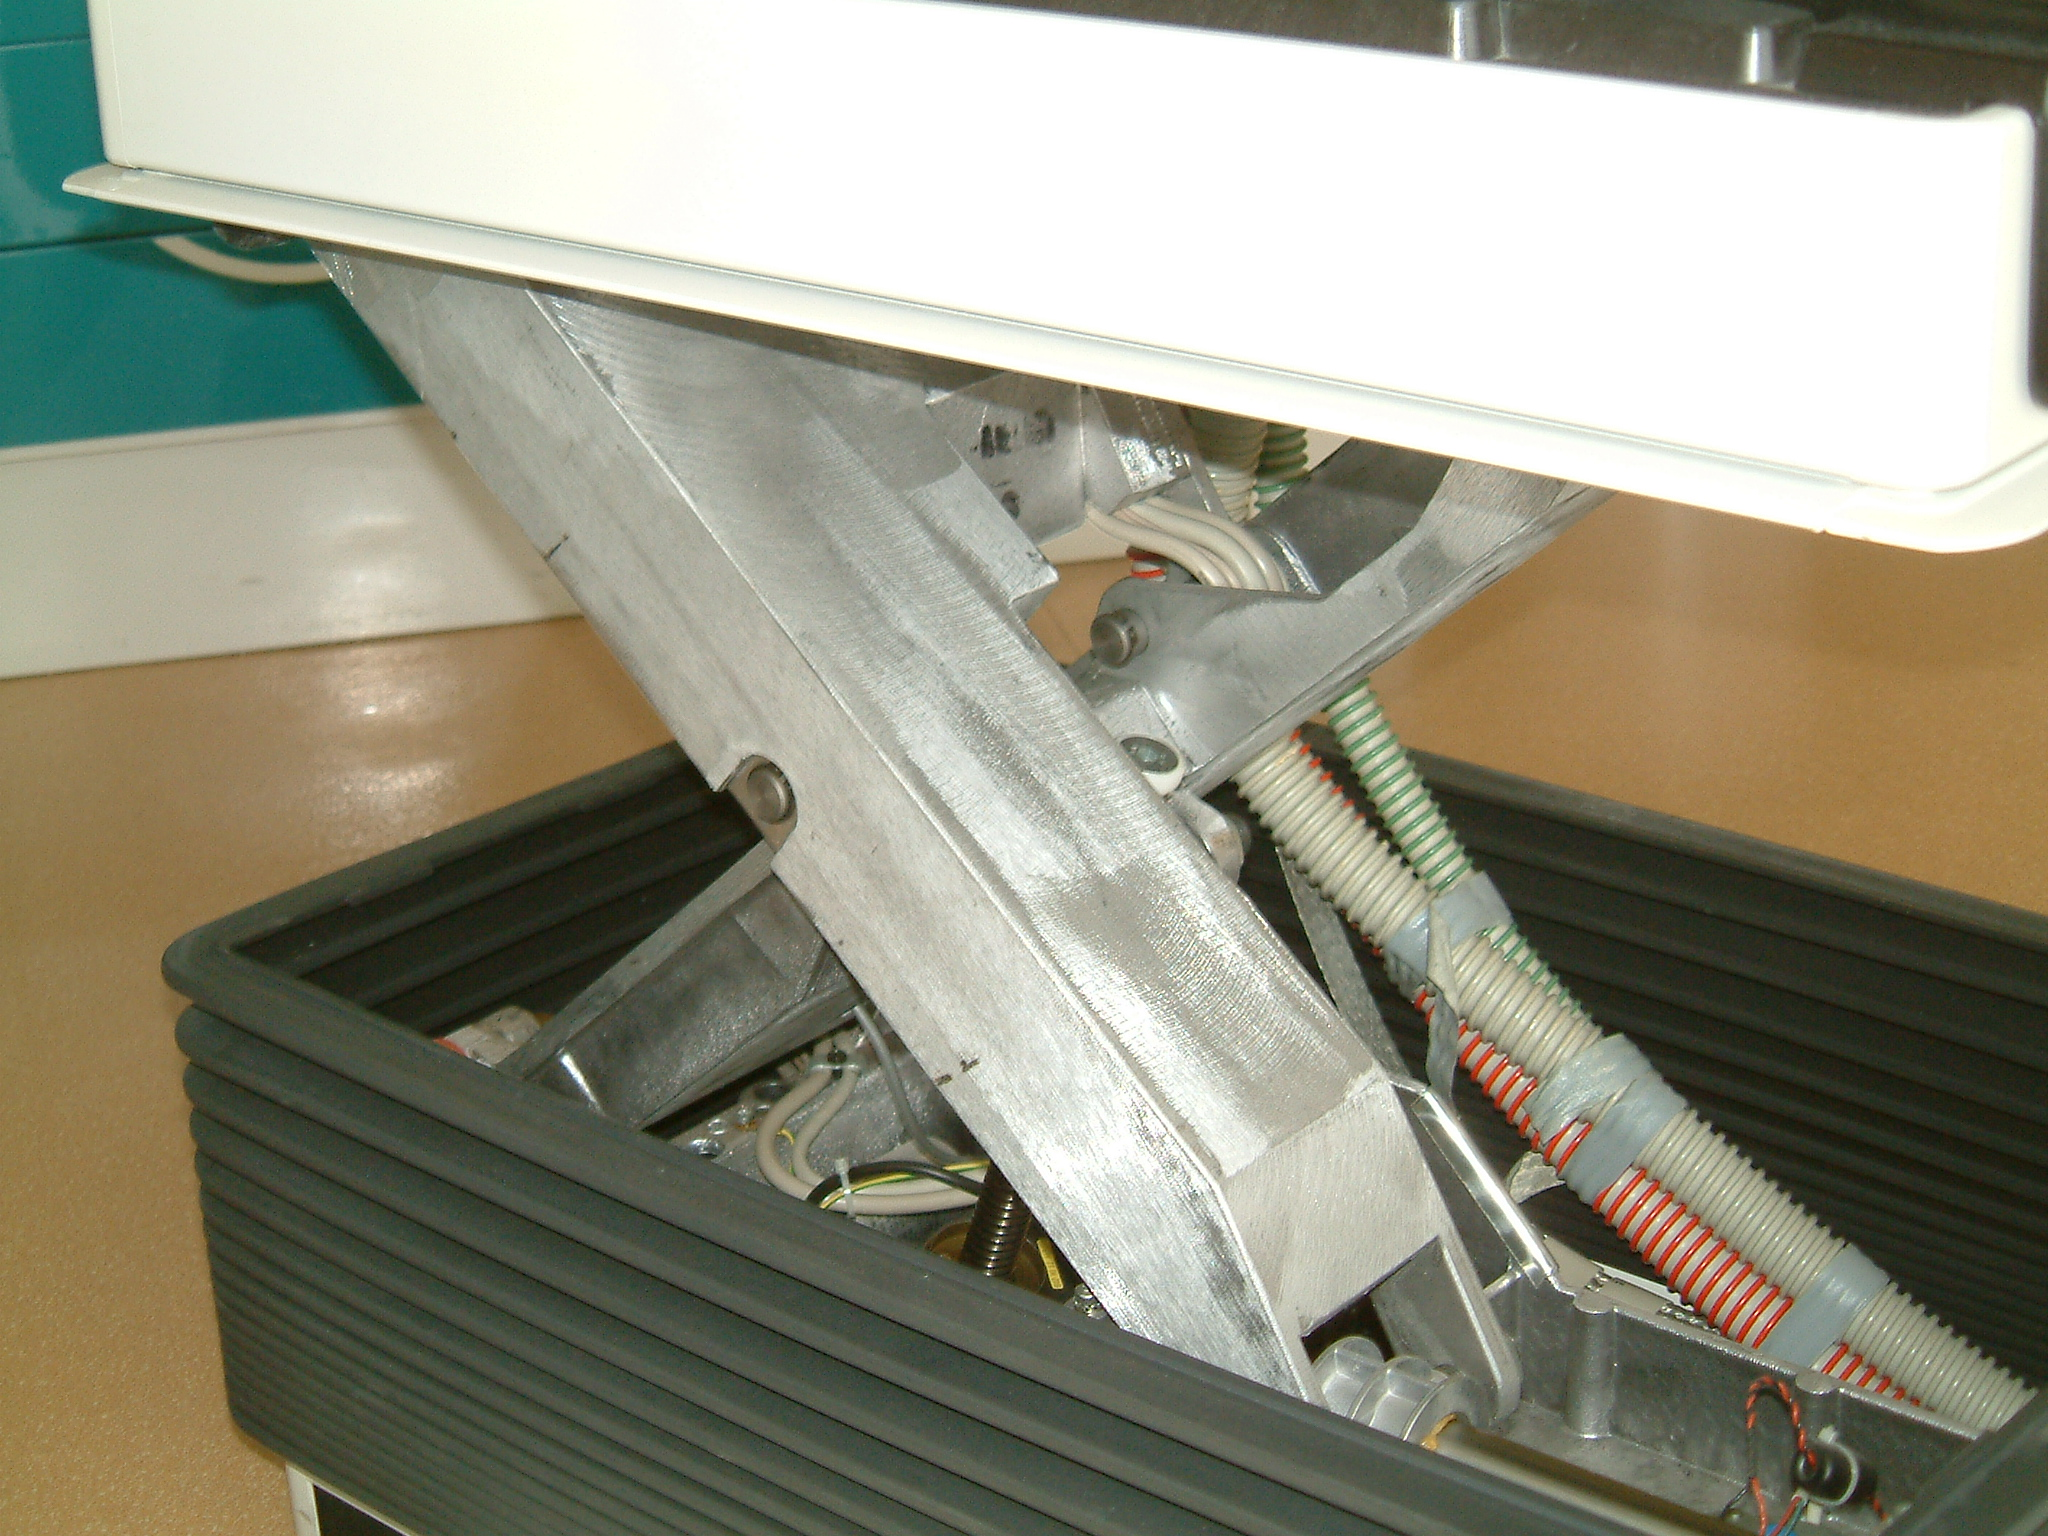
\includegraphics[width=\linewidth]{img/detail_chaise.png}
\caption{Système de levée}
\label{fig:image2}
\end{center}
\end{minipage}
\end{figure}

\newpage

\subsection{Descriptif de la cinématique}

La figure \ref{fig:image7}, montre les pièces du système numérotées.

\begin{itemize}
 \item La pièce 9 est en liaison pivot glissant avec la pièce 16, cette pièce est intégrée à la classe d'équivalence 1,
 \item La pièce 9' est en liaison pivot glissant avec la pièce/classe d'équivalence 5,
 \item La pièce 9' est en liaison pivot avec la pièce 3, la 9 avec la pièce/classe d'équivalence 4,
 \item Les pièces/classes d'équivalence 3 et 4 sont liées par une liaison pivot par l'intermédiaire des pièces 12 et 13, ces pièces sont intégrées à la classe d'équivalence 3,
 \item La pièce 8 est en liaison pivot avec la pièce 3 par l'intermédiaire des pièces 20, 21 et 27, ces pièces sont intégrées à la classe d'équivalence 3,
 \item Les pièces/classes d'équivalence 7 et 8 sont liées par une liaison hélicoïdale,
 \item La pièce 7 est liée au rotor du moteur dont le stator est numéroté 6. Cela signifie qu'il y a une liaison pivot entre ces pièces. La pièce 6 est elle est en liaison pivot par rapport à la pièce 1,
 \item La pièce 3 est en liaison pivot par rapport à la pièce 2 par l'intermédiaire de la pièce 22, ces pièces sont intégrées à la classe d'équivalence 2,
 \item La pièce 4 est en liaison pivot par rapport à la pièce 5. Les pièces 1 et 2 sont solidaires.
\end{itemize}

~\

Données géométriques:
\begin{itemize}
 \item $\overrightarrow{AB}=l(t).\overrightarrow{x_6}$,
 \item $\overrightarrow{AD}=a.\overrightarrow{x}+b.\overrightarrow{y}$,
 \item $\overrightarrow{DK}=L.\overrightarrow{x_3}$.
\end{itemize}



\begin{figure}[htbp]
\begin{center}
\includegraphics[width=\linewidth]{img/face.png}
\caption{Système de levée}
\label{fig:image7}
\end{center}
\end{figure}

\begin{figure}[htbp]
\begin{minipage}[c]{.55\linewidth}
\begin{center}
\includegraphics[width=\linewidth]{img/pos_haute.png}
\caption{Position haute}
\label{fig:image4}
\end{center}
\end{minipage}
\hfill
\begin{minipage}[c]{.4\linewidth}
\begin{center}
\includegraphics[width=\linewidth]{img/perspective.png}
\caption{Position intermédiaire}
\label{fig:image5}
\includegraphics[width=\linewidth]{img/pos_basse.png}
\caption{Position basse}
\label{fig:image6}
\end{center}
\end{minipage}
\end{figure}

\paragraph{Question 1:} Réaliser le graphe de liaison de ce mécanisme. Donner, pour chaque liaison, le type de liaison, le point d'application ainsi que le ou les axes nécessaires à sa description.

\paragraph{Question 2:} Représentez le mécanisme d'élévation du siège à l'aide d'un schéma cinématique.

\paragraph{Question 3:} Écrire le torseur de chacune de ces liaisons à son point d'application.

Le système présente la chaine de fermeture cinématique suivante:

\begin{math}
\left\{V_{3/1}\right\}=\left\{V_{3/8}\right\}+\left\{V_{8/7}\right\}+\left\{V_{7/6}\right\}+\left\{V_{6/1}\right\}
\end{math}

\paragraph{Question 4:} En déduire $\omega_{31}$ en fonction de $\omega_{76}$.

\paragraph{Question 5:} Déterminer la vitesse de montée du siège $V_{51}$ en fonction de $\theta_3$ et de $\omega_{31}$. Montrer qu'il est alors possible de connaître la vitesse de montée du siège en fonction de la vitesse de rotation du moteur.

\clearpage

\ifdef{\public}{\end{document}}

\pagestyle{correction}

\section{Correction}

\subsection{Moteur à explosion}

\paragraph{Question 1:} Graphe de liaison

\begin{minipage}{0.4\linewidth}
  \begin{itemize}
    \item 0: Bâti,
    \item 1: Vilebrequin,
    \item 2: Bielle,
    \item 3: Piston.
  \end{itemize}
\end{minipage}
\hfill
\begin{minipage}{0.4\linewidth}
 Graphe des liaisons
\end{minipage}

\paragraph{Question 2:} Schéma cinématique

\begin{center}
	\includegraphics[width=0.35\linewidth]{img/moteur_cin}
\end{center}

\paragraph{Question 3:}
$\left\{V_{A\in 1/0}\right\}=
\left\{\begin{array}{cc}
0 & 0 \\
0 & 0 \\
\omega_{10} & 0
\end{array}\right\}_{A,R}$
$\left\{V_{B\in 2/1}\right\}=
\left\{\begin{array}{cc}
0 & 0 \\
0 & 0 \\
\omega_{21} & 0
\end{array}\right\}_{B,R}$
$\left\{V_{C\in 3/2}\right\}=
\left\{\begin{array}{cc}
0 & 0 \\
0 & 0 \\
\omega_{32} & 0
\end{array}\right\}_{C,R}$
$\left\{V_{C\in 3/0}\right\}=
\left\{\begin{array}{cc}
0 & 0 \\
\omega_{30} & \omega_{30} \\
0 & 0
\end{array}\right\}_{C,R}$

\paragraph{Question 4:} $\overrightarrow{AB}=a.\overrightarrow{x_1}$, $\overrightarrow{BC}=b.\overrightarrow{x_2}$.

Avec $\left\{\begin{array}{l} \overrightarrow{x_1}=cos(\theta_1).\overrightarrow{x}+sin(\theta_1).\overrightarrow{y} \\ \overrightarrow{y_1}=-sin(\theta_1).\overrightarrow{x}+cos(\theta_1).\overrightarrow{y}\end{array}\right.$
$\left\{\begin{array}{l} \overrightarrow{x_2}=cos(\theta_2).\overrightarrow{x}+sin(\theta_2).\overrightarrow{y} \\ \overrightarrow{y_2}=-sin(\theta_2).\overrightarrow{x}+cos(\theta_2).\overrightarrow{y}\end{array}\right.$

\paragraph{Question 5:} $\overrightarrow{V_{C\in 3/2}}=\overrightarrow{0}$

$\overrightarrow{V_{C\in 2/1}}=\overrightarrow{V_{B\in 2/1}}+\overrightarrow{CB}\wedge \overrightarrow{\Omega_{2/1}}=-b.\overrightarrow{x_2}\wedge \omega_{21}.\overrightarrow{z}=b.\omega_{21}.\overrightarrow{y_2}$

$\overrightarrow{V_{C\in 1/0}}=\overrightarrow{V_{A\in 1/0}}+\overrightarrow{CA}\wedge \overrightarrow{\Omega_{1/0}}=-(b.\overrightarrow{x_2}+a.\overrightarrow{x_1})\wedge \omega_{10}.\overrightarrow{z}=\omega_{10}.(b.\overrightarrow{y_2}+a.\overrightarrow{y_1})$

\paragraph{Question 6:} $\overrightarrow{V_{C\in 3/0}}=a.\omega_{10}.\overrightarrow{y_1}+b.(\omega_{21}+\omega_{10}).\overrightarrow{y_2}$

\paragraph{Question 7:} $\overrightarrow{V_{C\in 3/0}}.\overrightarrow{x}=0$

\paragraph{Question 8:} 
\begin{itemize}
 \item $(a.\omega_{10}.\overrightarrow{y_1}+b.(\omega_{21}+\omega_{10}).\overrightarrow{y_2}).\overrightarrow{x}=0$,
 \item $(a.\omega_{10}.\overrightarrow{y_1}+b.(\omega_{21}+\omega_{10}).\overrightarrow{y_2}).\overrightarrow{y}=\|\overrightarrow{V_{C\in 3/0}}\|$.
\end{itemize}

Un ficher python permettant de tracer la vitesse du piston est disponible ici : \url{https://github.com/Costadoat/S04/raw/master/TD02/piston.py}

\subsection{Chaise de dentiste}

\paragraph{Question 1:} Graphe de liaison

\paragraph{Question 2:} Schéma cinématique

\begin{center}
	\includegraphics[width=0.7\linewidth]{img/chaise_cin}
\end{center}

\paragraph{Question 3:} 

$\left\{V_{9/1}\right\}=
\left\{\begin{array}{cc}
\omega_{91} & V_{91} \\
0 & 0 \\
0 & 0
\end{array}\right\}_{H,R}$
$\left\{V_{4/9}\right\}=
\left\{\begin{array}{cc}
0 & 0 \\
0 & 0 \\
\omega_{49} & 0
\end{array}\right\}_{H,R}$
$\left\{V_{3/1}\right\}=
\left\{\begin{array}{cc}
0 & 0 \\
0 & 0 \\
\omega_{31} & 0
\end{array}\right\}_{D,R}$
$\left\{V_{4/3}\right\}=
\left\{\begin{array}{cc}
0 & 0 \\
0 & 0 \\
\omega_{43} & 0
\end{array}\right\}_{C,R}$
$\left\{V_{9'/3}\right\}=
\left\{\begin{array}{cc}
0 & 0 \\
0 & 0 \\
\omega_{9'3} & 0
\end{array}\right\}_{K,R}$
$\left\{V_{5/9'}\right\}=
\left\{\begin{array}{cc}
\omega_{59'} & V_{59'} \\
0 & 0 \\
0 & 0
\end{array}\right\}_{K,R}$
$\left\{V_{6/1}\right\}=
\left\{\begin{array}{cc}
0 & 0 \\
0 & 0 \\
\omega_{61} & 0
\end{array}\right\}_{A,R}$
$\left\{V_{8/7}\right\}=
\left\{\begin{array}{cc}
\omega_{87} & V_{87} \\
0 & 0 \\
0 & 0
\end{array}\right\}_{A,R_6}$, avec $V_{87}=\frac{pas}{2\pi}.\omega_{87}$ \\
$\left\{V_{7/6}\right\}=
\left\{\begin{array}{cc}
\omega_{76} & 0 \\
0 & 0 \\
0 & 0
\end{array}\right\}_{A,R_6}$
$\left\{V_{3/8}\right\}=
\left\{\begin{array}{cc}
0 & 0 \\
0 & 0 \\
\omega_{38} & 0
\end{array}\right\}_{B,R}$

\paragraph{Question 4:}

\begin{math}
\left\{V_{3/1}\right\}=\left\{V_{3/8}\right\}+\left\{V_{8/7}\right\}+\left\{V_{7/6}\right\}+\left\{V_{6/1}\right\}
\end{math}

Déplacement des torseurs au point A.

$\left\{V_{3/8}\right\}=
\left\{\begin{array}{cc}
0 & 0 \\
0 & 0 \\
\omega_{38} & 0
\end{array}\right\}_{B,R}=
\left\{\begin{array}{cc}
0 & 0 \\
0 & -l(t).\omega_{38} \\
\omega_{38} & 0
\end{array}\right\}_{A,R_6}$

$\left\{V_{3/1}\right\}=
\left\{\begin{array}{cc}
0 & 0 \\
0 & 0 \\
\omega_{31} & 0
\end{array}\right\}_{D,R}=
\left\{\begin{array}{cc}
0 & b.\omega_{31} \\
0 & -a.\omega_{31} \\
\omega_{31} & 0
\end{array}\right\}_{A,R}$


\begin{math}
\left\{\begin{array}{cc}
0 & b.\omega_{31} \\
0 & -a.\omega_{31} \\
\omega_{31} & 0
\end{array}\right\}_{A,R}=
\left\{\begin{array}{cc}
0 & 0 \\
0 & -l(t).\omega_{38} \\
\omega_{38} & 0
\end{array}\right\}_{A,R_6}+
\left\{\begin{array}{cc}
\omega_{87} & V_{87} \\
0 & 0 \\
0 & 0
\end{array}\right\}_{A,R_6}+
\left\{\begin{array}{cc}
\omega_{76} & 0 \\
0 & 0 \\
0 & 0
\end{array}\right\}_{A,R_6}+
\left\{\begin{array}{cc}
0 & 0 \\
0 & 0 \\
\omega_{61} & 0
\end{array}\right\}_{A,R}
\end{math}

\begin{eqnarray}
\omega_{31}.\overrightarrow{z}=\omega_{38}.\overrightarrow{z_6}+\omega_{87}.\overrightarrow{x_6}+\omega_{76}.\overrightarrow{x_6}+\omega_{61}.\overrightarrow{z} \label{eq:chaise1} \\
b.\omega_{31}.\overrightarrow{x}-a.\omega_{31}.\overrightarrow{y}=-l(t).\omega_{38}.\overrightarrow{y_6}+V_{87}.\overrightarrow{x_6} \label{eq:chaise2} 
\end{eqnarray}

En sachant que $\overrightarrow{z}=\overrightarrow{z_6}$, on obtient en projetant \ref{eq:chaise1} sur $\overrightarrow{x_6}$, puis sur $\overrightarrow{z}=\overrightarrow{z_6}$:

\begin{eqnarray}
\omega_{31}=\omega_{38}+\omega_{61} \label{eq:chaise3} \\
0=\omega_{87}+\omega_{76} \label{eq:chaise4} 
\end{eqnarray}

En projetant \ref{eq:chaise2} sur $\overrightarrow{x}$, puis sur $\overrightarrow{y}$ après avoir fait un changement de repère, on obtient:

\begin{eqnarray}
b.\omega_{31}=l(t).sin\theta_6.\omega_{38}+\frac{p}{2.\pi}.\omega_{87}.cos\theta_6 \label{eq:chaise5} \\
-a.\omega_{31}=-l(t).cos\theta_6.\omega_{38}+\frac{p}{2.\pi}.\omega_{87}.sin\theta_6 \label{eq:chaise6}
\end{eqnarray}

En écrivant isolant les $\omega_{38}$ et en divisant \label{eq:chaise5} par \label{eq:chaise6}, on obtient:

\begin{eqnarray}
\frac{sin \theta_6}{cos \theta_6}=\frac{b.\omega_{31}-\frac{p}{2.\pi}.\omega_{87}.cos\theta_6 }{a.\omega_{31}+\frac{p}{2.\pi}.\omega_{87}.sin\theta_6} \label{eq:chaise7}
\end{eqnarray}

Soit:

\begin{eqnarray}
b.cos \theta_6.\omega_{31}-\frac{p}{2.\pi}.\omega_{87}.cos\theta_6^2=a.sin \theta_6.\omega_{31}+\frac{p}{2.\pi}.\omega_{87}.sin\theta_6^2 \label{eq:chaise8}
\end{eqnarray}

Donc:

\begin{eqnarray}
\omega_{31}=\frac{\frac{p}{2.\pi}}{a.sin\theta_6-b.cos\theta_6}.\omega_{76} \label{eq:chaise9}
\end{eqnarray}

\paragraph{Question 5:}

HDEK est un rectangle donc les côtés HD et KE sont toujours parallèles donc le mouvement de 5/1 est une translation, donc: $\overrightarrow{V_{E\in5/1}}=\overrightarrow{V_{K\in5/1}}$, de plus la direction (DE) est toujours verticale donc cette translation est verticale, donc $\overrightarrow{V_{E\in5/1}}=V_{51}.\overrightarrow{y}$.

$\overrightarrow{V_{K\in5/1}}=\overrightarrow{V_{K\in5/9'}}+\overrightarrow{V_{K\in9'/3}}+\overrightarrow{V_{K\in3/1}}$, or la liaison entre 9' et 3 est une pivot d'axe $(C,\overrightarrow{z})$, donc $\overrightarrow{V_{K\in9'/3}}=\overrightarrow{0}$.

La liaison 5/9' est une pivot glissant d'axe $(K,\overrightarrow{x})$, donc $\overrightarrow{V_{K\in5/9'}}=V_{59'}.\overrightarrow{x}$.

Ainsi, $\overrightarrow{V_{K\in5/1}}.\overrightarrow{y}=V_{51}=\overrightarrow{V_{K\in3/1}}.\overrightarrow{y}$

$V_{51}=(\overrightarrow{V_{D\in3/1}}+\overrightarrow{KD}\wedge \overrightarrow{\omega_{31}}).\overrightarrow{y}=(\overrightarrow{KD}\wedge \overrightarrow{\omega_{31}}).\overrightarrow{y}$

$V_{51}=(-L.\overrightarrow{x_3}\wedge \omega_{31}.\overrightarrow{z}).\overrightarrow{y}$

$V_{51}=L.\omega_{31}\overrightarrow{y_3}.\overrightarrow{y}$

$V_{51}=L.cos\theta_3.\omega_{31}$

%Un ficher python permettant de tracer la vitesse de montée du siège est disponible ici : \url{https://github.com/Costadoat/S04/raw/master/TD02/siege_dentiste.py}

\end{document}
